\documentclass[a4paper,twoside,12pt]{book}
\renewcommand{\baselinestretch}{1.7}
\usepackage[utf8]{inputenc}
\usepackage{natbib}
\usepackage{graphicx}
\usepackage[a4paper, left=37mm, right=27mm, top=39mm, bottom=39mm, headsep=12mm, footskip=15mm]{geometry}
\setlength{\headheight}{15pt}
\usepackage{fancyhdr}
\usepackage{fontenc}
\usepackage{float}
\usepackage{rotating}
\usepackage{hyperref}
\usepackage{afterpage}
\usepackage{mathtools}
\usepackage{amsmath}
\usepackage{amssymb}
\usepackage{tabu}
\usepackage{listings}
\usepackage{subcaption}
\usepackage{emptypage}
\usepackage{bookmark}
\usepackage{xfrac}
\usepackage{epsfig}
\usepackage{listings}
\usepackage{url}
\usepackage{bm}

\setlength{\parskip}{1em}

\makeatletter
\g@addto@macro\normalsize{%
  \setlength\abovedisplayskip{20pt}
  \setlength\belowdisplayskip{40pt}
  \setlength\abovedisplayshortskip{20pt}
  \setlength\belowdisplayshortskip{40pt}
}

\lstset{ %
  basicstyle=\footnotesize
}

\pagestyle{fancy}
\renewcommand{\chaptermark}[1]{\markboth{#1}{}}
\renewcommand{\sectionmark}[1]{\markright{\thesection\ #1}}
\fancyhf{} \fancyhead[LE,RO]{\bfseries\thepage}
\fancyhead[LO]{\bfseries\rightmark}
\fancyhead[RE]{\bfseries\leftmark}
\renewcommand{\headrulewidth}{0.5pt}
\renewcommand{\footrulewidth}{0pt}
\fancypagestyle{plain}{
	\fancyhead{}
	\renewcommand{\headrulewidth}{0pt}}

%%%%%%%%%% General thesis informations go here! (TITLE, AUTHOR-NAME, KEYWORD-1, KEYWORD-2,...
\hypersetup{
    pdfauthor  = {Delbono Alex},    		    % author
    pdftitle   = {Consensus based control for a Unmanned Aerial Vehicle formation},    				% title
 	pdfsubject = {Master's Degree Thesis},  % subject of the document
 	pdfkeywords= {Consensus, UAVs, Formation}      % list of keywords
}

%%%%%%%%%%%%%%%%%%%%%%%%%%%%%% BEGIN OF THE DOCUMENT
\begin{document}

\pagestyle{fancy}
\renewcommand{\chaptermark}[1]{\markboth{#1}{}}
\renewcommand{\sectionmark}[1]{\markright{\thesection\ #1}}
\fancyhf{} \fancyhead[LE,RO]{\bfseries\thepage}
\fancyhead[LO]{\bfseries\rightmark}
\fancyhead[RE]{\bfseries\leftmark}
\renewcommand{\headrulewidth}{0.5pt}
\renewcommand{\footrulewidth}{0pt}
\fancypagestyle{plain}{
	\fancyhead{}
	\renewcommand{\headrulewidth}{0pt}}

%%%%%%%%%%%%%%%%%%%%%%%%%%%%%% Title page
\newgeometry{margin=3cm}
\begin{titlepage}

%%%%%%%%%% Department informations go here!
\begin{center}
\Large{\textsc{Politecnico di Milano}}\\
\Large{School of Industrial and Information Engineering}\\
\large{Computer Science and Engineering Course}\\
\large{Dipartimento di Elettronica, Informazione e Bioingegneria}
\par
\end{center}

\vspace{0.2cm}

\begin{center}
\begin{figure}[h]
\centering{}
\includegraphics[width=0.3\textwidth]{title-page/logo-polimi}
\end{figure}
\par
\end{center}

%%%%%%%%%% Thesis title goes here!
\begin{center}
\LARGE{Consensus algorithm \\for a formation of Unmanned Aerial Vehicles}
\vspace{1.0cm}
\par
\end{center}

%%%%%%%%%% Advisor and co-advisor names go here!
\begin{flushleft}
\begin{tabular}{ll}
Advisor:  & Prof. Marco LOVERA\tabularnewline
Co-Advisor:  & Prof. Name SURNAME\tabularnewline
\end{tabular}\vspace{0.5cm}
\par
\end{flushleft}

%%%%%%%%%% Student name goes here!
\begin{flushright}
\begin{tabular}{ll}
Thesis by: & \tabularnewline
Alex DELBONO & Matr. 850114\tabularnewline
\end{tabular}\vspace{1cm}
\par
\end{flushright}

\begin{center}
{\large{}Academic Year 2016\textendash 2017}
\par
\end{center}{\large \par}

\end{titlepage}

\restoregeometry

\cleardoublepage{}

%%%%%%%%%%%%%%%%%%%%%%%%%%%%%% Dedication
\begin{flushright}
\emph{A Pietro, una persona vera ed altruista come poche\ldots{}
}
\cleardoublepage{}
\par
\end{flushright}

%%%%%%%%%%%%%%%%%%%%%%%%%%%%%% Acnowledgment
\chapter*{Ringraziamenti}
\addcontentsline{toc}{chapter}{Ringraziamenti}
%«È di cattivo gusto ringraziare il relatore. Se vi ha aiutato ha fatto solo il suo dovere» Uberto Eco, Come si fa una tesi di laurea

Al termine del mio percorso di studi, vorrei porgere i miei più profondi ringraziamenti
a tutte le persone che hanno contribuito, in misura più o meno significativa, alla mia
crescita professionale e personale.
Inizio ringraziando la mia famiglia, il cui supporto economico e morale non è mai mancato.
In particolare, sono estremamente grato a mia madre per avermi dato la possibilità
di focalizzarmi sull’università, investendo parte del suo tempo per offrirmi
le migliori condizioni di studio possibili.
Ringrazio mio padre, per gli insegnamenti che mi ha trasmesso e per come, mediante l’esempio,
mi ha mostrato ad affrontare le sfide con passione e tenacia.
Un pensiero particolare va a Ilaria, mia sorella, una donna con dei sani valori,
testarda e irascibile come poche, ed in grado di raggiungere grandi traguardi.
Mi auguro che possa ricevere dalla vita i premi del duro lavoro che ha compiuto e che sarà chiamata a svolgere.
Ringrazio Antonio, mio compagno d’avventure in questi anni, per tutte le
esperienze vissute insieme e, soprattutto, per non essere mai mancato nei momenti di difficoltà.
Un grazie va poi ad Andrea, che è stato una presenza costante nella mia permanenza milanese,
un uomo sempre disponibile per un consiglio e sempre pronto a tendermi la mano.
Ringrazio Iris per la pazienza dimostrata e le sono grato per l’energia che è
riuscita a trasmettermi.
Le auguro il meglio per la sua vita e sono sicuro che sarà capace di raggiungere
tutti i traguardi che si è prefissata.
Non posso non considerare l’aiuto indispensabile che Veronica ha voluto darmi in questi mesi.
Nonostante la mole di lavoro a cui era sottoposta, ha saputo trovare tempo da dedicarmi.
Vorrei quindi ringraziarla profondamente.
Porgo i miei sentiti ringraziamenti al professor Lovera, per avermi accompagnato
durante la stesura della tesi e per la pazienza dimostrata in alcune occasioni.
Lo ringrazio per la stima e per la fiducia che ha riposto in me.
Un ringraziamento va a Mattia, che mi ha fornito un supporto indispensabile
nello svolgimento pratico della tesi, offrendomi le sue competenze ingegneristiche
e la sua esperienza con i droni.
Infine, vorrei ringraziare Pietro per tutto ciò che ha fatto per me.
Non si è rivelato solamente un supervisore, ma ha saputo essere un punto saldo
a cui sorreggersi nei momenti difficili. Lo ringrazio di cuore
per il suo altruismo disinteressato e non dimenticherò mai quello che ha fatto per me. 


%%%%%%%%%%%%%%%%%%%%%%%%%%%%%% Abstract
\chapter*{Abstract}
\addcontentsline{toc}{chapter}{Abstract}
%The abstract must contain 3 main logic blocks which will be discussed in the introduction.

%Field of work
%The first block must contain a sentence which describes the field of work, and eventually another sentence which focuses the specific objective of the work in details.

%Purpose of the thesis
%The second block must start with the words «The purpose of the thesis is …».

%Short recap
%The last block must summarize the conducted activities and the obtained results (evaluating them eventually).

This thesis is about the synchronized flight of a formation of multirotors which executes a mission.
The mission is characterized by a trajectory for every drone which composes the formation.
The formation must be able to deal with unforeseen events, which can compromise
the outcome of the mission. In order to do that, the drones must exchange information
between each others, therefore a support network is needed.

The purpose of this thesis is to present the algorithm for synchronized formation flight
called “Consensus algorithm” and implement it in a simulated environment
and in a real system with heterogeneous drones. We want to verify that the theoretical
results can be applied in a real distributed system, with not ideal network performances.

In the first part, we explain the algorithm used during the experimental work,
while in the following chapter the software and hardware used are presented.
In the last chapters we show in detail the structure of the software and the experiment conducted.
In particular, many simulations will be presented to confirm the quality of the
“Consensus algorithm”. Finally, a comparison between the simulated results and the ones
obtained in the real environment is proposed.


%%%%%%%%%%%%%%%%%%%%%%%%%%%%%% Sommario
\chapter*{Sommario}
\addcontentsline{toc}{chapter}{Sommario}
%Il testo delle tesi redatte in lingua straniera dovrà essere introdotto da un ampio estratto in lingua italiana, che andrà collocato dopo l’abstract.

La tesi tratta di volo sincronizzato di una formazione di multirotori che eseguono una missione,
caratterizzata da una traiettoria per ogni drone che compone la formazione.
La formazione deve essere in grado di reagire a eventi inaspettati, che posssono
compromettere l'esito della missione stessa.
Per raggiungere tale scopo, i droni devono scambiare informazioni, attraverso
una rete di supporto.

L'obbiettivo della tesi è di presentare l'algoritmo utilizzato per il volo sincronizzato,
chiamato “Algoritmo di Consenso” e implementarlo sia in un ambiente simulato,
che in un sistema reale, composto da macchine eterogenee. Si vuole verificare che
i risultati teorici possano essere applicati in un sistema reale distribuito, dotato di
una rete di comunicazione dalle prestazioni non ideali.

Nella prima parte della tesi, verrà esposto l'algoritmo usato durante il lavoro sperimentale,
mentre nel capitolo seguente saranno presentati l'hardware e il software.
Negli ultimi capitoli saranno evidenziati nel dettaglio la struttura del software
e gli esperimenti condotti.
In praticolare, saranno mostrate alcune simulationi, in modo da confermare la bontà
dell'“Algoritmo di Consenso”.
Infine, nell'ultimo capitolo, sarà proposta una comparazione tra i risultati
delle simulazioni e quelli ottenuti mediante l'implementazione in un sistema reale.


%%%%%%%%%%%%%%%%%%%%%%%%%%%%%% Table of contents
\tableofcontents

%%%%%%%%%%%%%%%%%%%%%%%%%%%%%% List of figures
\listoffigures
\addcontentsline{toc}{chapter}{List of figures}
\cleardoublepage{}

%%%%%%%%%%%%%%%%%%%%%%%%%%%%%% Introduction
\chapter*{Introduction\label{chap:introduction}}
\addcontentsline{toc}{chapter}{Introduction}
\markboth{Introduction}{Introduction}
%The introduction must be atomic, it does not have to include subsections nor paragraphs.

%The title, the abstract and the introduction must appear as chinese boxes: if read in this order, they must progressively show the informations about the topic in order to catch the attention of the reader.

%The introduction must be divided in three main logic blocks as well:
%General overview
%A brief description of the work
%Structure of the thesis

In recent years, the field of robotics had developed rapidly.
The growing applications of mobile robots and drones in many fields
has brought an important increase in the number of robotic vehicles.
Many commercial solutions are available, but, in many cases, they offer
a product which needs an expert pilot. For this reason and due to the high prices,
the diffusion of mobile robots is limited. In the latest years, these problems were
mitigated and we now find lower prices and easier-to-use products. This will boost
the diffusion of non-professional robotic vehicles in our houses and in our daily activities.
Applications of UAVs are the ones are the ones related to exploration and data
collection. Indeed, drones are fundamental in inspection of unknown areas, such as
forests or unreachable terrains.
Moreover, the monitoring of industrial artifacts constitutes a valuable application of UAVs,
such as for instance, solar panels, wind turbines, high-voltage cables or tubes can be
supervised using aerial vehicles.
The multimedia production is the field in which the drones are most present. Indeed,
most of the machines are equipped with high-definition cameras in order to provide
professional videos.

The power consumptions of the machines has been significantly reduced in the recent years
and we are now able to build smaller and lighter vehicles.
In particular, in the aerial field there are commercial products which weight
about 200g with a flight time of 20 minutes.
These improvements allow us to develop more advanced features, such as
trajectory planning, obstacles avoidance, formation flight.
The development of autonomous UAVs is fundamental for humanitarian
response around the world. When a natural calamity happens, the UAVs can play a
crucial role by delivering essential goods or finding missing people. Moreover, the
operations can be done without risking the safety or the life of the rescuers, because
they can act remotely or plan an autonomous mission.

The trajectory planning is essential for the development of autonomous vehicles,
because the generation of a feasible trajectory for a mission is required,
otherwise no mission can be done.
The trajectory generation is a difficult problem, because of its computational complexity.
Indeed, many suboptimal algorithms have been developed in order to reduce this
complexity.
There are different classes of planning algorithm and they can be summarized as follows:
\begin{itemize}
  \item Artificial Potential Field: these algorithms assign a value of the potential
  for every point in the map. The goal has the lowest (highest) value and the obstacles
  have high (low) values. Then, the robot tries to descend (climb) the potential,
  in order to reach the goal.

  \item Sampling Based Planning: random samples are used to find a path from the
  starting point to the goal. Advanced random samples techniques can be used in order
  to reduce the complexity of the algorithm.

  \item Grid Based Planning: this kind of algorithm overlays a grid on the map, so
  every configuration corresponds with a grid pixel.
  The robot can move from one grid pixel to any adjacent grid pixels as long
  as that grid pixel does not contain an obstacle.

  \item Reward-Based Planning: the robot can apply different actions in every state
  of the world. The outcome of an action can be not deterministic and after every
  action, the robot gains a reward. The objective of the robot is to maximize the
  sum of the rewards.
\end{itemize}

Another important aspect is the obstacle avoidance. The trajectory is usually planned
offline, when the mission is not started yet. So, the trajectory does not take into
account the fact that an unplanned obstacle might interfere with the mission. In this
case another algorithm is implemented to run online. This kind of algorithms
are called obstacle avoidance algorithms and they plan again locally the trajectory, in
order to get rid of unforeseen events. These algorithms need the drone to be equipped
with proximity sensors, which provide information about the surrounding environment.
Different methodologies have been developed for obstacles avoidance. The main ones are
summarized below without details.

\begin{itemize}
  \item Artificial Potential Field: as before, the idea of this approach is that
  obstacles exert a virtual repulsive force, given by the potential field, to push
  away the robot from them while the goal position generates a virtual attractive
  force to guide the robot to it.

  \item Virtual Force Field method (VFF): is the combination of the Artificial Potential
  Field with the concept of Probabilistic Occupancy Grid maps.

  \item Fuzzy Controller for Obstacle Avoidance: as the name says, a fuzzy controller
  is used to derive the variables for the vehicle’s orientation and acceleration control,
  depending on the current perception of the robot’s sensors

  \item Vector Field Histogram method (VFH): improved version of the VFF method.

  \item VFH+, VFH$^*$ method: improved versions of the VFH method, but more computational costly.
  The most recent one is the VFH method, which uses an A$^*$ search.

  \item Traversability Field Histogram (TFH): The local path planner bases on
  the VFH concept, but is extended by the information provided within the Traversability Map.

  \item Dynamic Window Approach: the algorithm takes into account the dynamic and kinematic constraints
  of the robot and it is similar to the VFH+ algorithm. The method is called
  dynamic window approach and considers only admissible velocities which can be
  reached within the next time interval and which allow the robot to stop safely.

  \item Curvature Velocity Space method: This method chooses a point in the linear-angular
  velocity space which satisfies some constraints and maximizes an objective function.
  This objective function tries to move the robot close to the commanded direction at
  the highest feasible speed, while travelling the trajectory with the largest clearance from obstacles.

  \item Beam Curvature method: improvement for the curvature velocity space method.

  \item Nearness diagram Navigation: it is similar to the VFH method, but uses
  a polar histogram to derive actions to be taken for the robot.
\end{itemize}

When multiple machines have to fly in a formation, a synchronization mechanism is
needed. For example, if one of the drones has to deviate from the planned trajectory
(for instance, because of an unplanned obstacle), the formation must be preserved.
To reach the synchronization, vehicles must communicate with each other and
exchange information.
Notions from graph theory are needed to analyze the behaviour of the system
and demonstrate the convergence properties.

This work is focused on the presentation of a distributed synchronization algorithm,
which we call consensus algorithm. Every drone must exchange its mission progression
with its neighbors and must adjust its mission progression based on the information
received from the other vehicles.
The algorithm is a distributed algorithm and it is executed on every vehicle.


In the first chapter, we will see the theoretical aspects of the consensus algorithm and then,
in the second chapter, we will provide a general overview of the hardware and software used to deploy the algorithm.
In the third chapter we will take a look at the software implementation of the main part of the
system, providing classes and snippets of code.
Finally, we will explain the simulated and experimental results of our work
in chapters four and five.
We will apply the algorithm to a real system and we will present our results and its
performances.


%%%%%%%%%%%%%%%%%%%%%%%%%%%%%% Chapter 1
\chapter{Consensus theory\label{chap:consensus_theory}}
\input{chapters/chapter-01/consensus_theory.tex}

%%%%%%%%%%%%%%%%%%%%%%%%%%%%%% Chapter 2
\chapter{System architecture\label{chap:system_architecture}}
In this chapter, we describe the hardware and software architecture of the system.
Most of the software is completely decoupled by the hardware part and can be run
on different machines, allowing portability and reusability. On the contrary, some
code is developed only for the specific hardware; mostly the code more related with
the specific functionalities of the hardware itself. We will have an overview of the hardware
used and then we show a general software architecture and its deployment on the
machines involved.

%% Sections of the chapter
\section{Hardware}

The hardware used to run the system is heterogeneous and we will show in details
the machines involved in the project.

First of all, we used a desktop pc as a ground station. It specifics are listed below:
\begin{itemize}
  \item Processor: Intel Core(TM) i5-6500 CPU @ 3.20GHz
  \item Memory: 16 GB
  \item Network: Intel Gigabit CT Network Adapter
  \item Storage: 230 GB
\end{itemize}

On this machine, we run a virtual machine which has the following specifics:
\begin{itemize}
  \item Processor: 1 Core
  \item Memory: 4 GB
  \item Storage 25 GB
  \item Network: Virtual adapter
\end{itemize}

The flying machines involved in the mission are of two kinds, but both adopt the
same general configuration, even with different hardware. Indeed, they are equipped
with a flight control unit connected with a companion microcomputer by the serial port
The microcomputer communicates with the ground station using the Wifi.

\subsection{Pixfalcon}
The flight control unit adopted it the Pixfalcon (figure \ref{fig:hardware_pixfalcon})
which belongs to the family of the Pixhawk \cite{pixhawk}.

\begin{figure}[h]
\centering
\includegraphics[width=0.35\textwidth]{chapters/chapter-03/figures/hardware_pixfalcon.png}
\caption{Pixfalcon board}
\label{fig:hardware_pixfalcon}
\end{figure}

Its specifications are the following:
\begin{itemize}
  \item Main System-on-Chip: STM32F427
        \begin{itemize}
          \item CPU: 180 MHz ARM Cortex M4 with single-precision FPU
          \item RAM: 256 KB SRAM (L1)
        \end{itemize}

  \item Failsafe System-on-Chip: STM32F100
        \begin{itemize}
          \item CPU: 24 MHz ARM Cortex M3
          \item RAM: 8 KB SRAM
        \end{itemize}

  \item Wifi: ESP8266 external
  \item GPS: U-Blox 7/8 (Hobbyking) / U-Blox 6 (3D Robotics)
  \item Connectivity:
    \begin{itemize}
      \item 1x I2C
      \item 1x CAN (2x optional)
      \item 1x ADC
      \item 4x UART (2x with flow control)
      \item 1x Console
      \item 8x PWM with manual override
      \item 6x PWM / GPIO / PWM input
      \item S.BUS / PPM / Spektrum input
      \item S.BUS output
    \end{itemize}
\end{itemize}

\subsection{Intel Edison}
The companion computers are of two types.
The first kind is the Intel Edison \cite{edison} (figure \ref{fig:hardware_edison})
which is a general purpose computer.

\begin{figure}[h]
\centering
\includegraphics[width=0.35\textwidth]{chapters/chapter-03/figures/hardware_edison.png}
\caption{Edison board}
\label{fig:hardware_edison}
\end{figure}

The specifications are the following:

\begin{itemize}
  \item Atom 2-Core (Silvermont) x86 @ 500 MHz
  \item Memory: LPDDR3 1 GB
  \item Storage: 4 GB EMMC
\end{itemize}

\subsection{RaspberryPi Zero}
The second kind of companion is the RaspberryPi Zero \cite{raspberry}
(figure \ref{fig:hardware_raspberry}).

\begin{figure}[h]
\centering
\includegraphics[width=0.35\textwidth]{chapters/chapter-03/figures/hardware_raspberry.jpg}
\caption{RaspberryPi Zero board}
\label{fig:hardware_raspberry}
\end{figure}

The specifications are the following:

\begin{itemize}
  \item Processor:
        \begin{itemize}
          \item Broadcom BCM2835
          \item contains an ARM1176JZFS (ARM11 using an ARMv6-architecture core)
        \end{itemize}

  \item Memory: 512MB LPDDR2 SDRAM

  \item USB On-The-Go port
  \item Mini HDMI
  \item 40pin GPIO header
  \item CSI camera connector (newer version from May 2016)
\end{itemize}

\subsection{Motive Optitrack}
The motion capture system is Motive Optitrack \cite{optitrack}.
We use eight Optitrack Prime 13 cameras \cite{prime13},
arranged on a square as show in the figure \ref{fig:camera_square}.

\begin{figure}[h]
\centering
\includegraphics[width=1.0\textwidth]{chapters/chapter-03/figures/cameras_square.png}
\caption{Motive Optitrack screenshot}
\label{fig:camera_square}
\end{figure}

The cameras are connected to a Netgear Prosafe 28PT GE POE \cite{netgear} switch using
Gigabit Ethernet cables.

In order to be visible by the Optitrack system, every drone must be equipped with
markers (figure \ref{fig:marker}), with different configurations,
which make possible the diversification of all the drones. %TODO photo markers

\begin{figure}[h]
\centering
\includegraphics[width=0.7\textwidth]{chapters/chapter-03/figures/marker.jpg}
\caption{Optitrack marker}
\label{fig:marker}
\end{figure}

The two models of drone which we will use are presented in the figures \ref{fig:ant1}
and \ref{fig:hexa}. The first one is the Ant model, which is equipped with the Raspberry
Pi Zero and the Pixfalcon. It is a tiny drones which weights about 200g.
The second one is the Hexa model. It is provided with the Intel Edison board and
the Pixfalcon. It is larger and its diameters is about 40cm long.
As we can see from the figures, the Ant model has four propellers, while the Hexa
is provided with six ones.

\begin{figure}[!htb]
\minipage{0.5\textwidth}
  \includegraphics[width=\linewidth]{chapters/chapter-03/figures/ant1_1.jpg}
\endminipage\hfill
\minipage{0.5\textwidth}
  \includegraphics[width=\linewidth]{chapters/chapter-03/figures/ant1_2.jpg}
\endminipage
\caption{Ant drone}
\label{fig:ant1}
\end{figure}

\begin{figure}[!htb]
\minipage{0.5\textwidth}
  \includegraphics[width=\linewidth]{chapters/chapter-03/figures/hexa_1.jpg}
\endminipage\hfill
\minipage{0.5\textwidth}
  \includegraphics[width=\linewidth]{chapters/chapter-03/figures/hexa_2.jpg}
\endminipage
\caption{Hexa drone}
\label{fig:hexa}
\end{figure}


\section{Software}

We now list all the software adopted in order to execute the algorithm
in a real environment and in the simulated one.

The principal software used to manage the distributed architecture is ROS Kinetic
Kame \cite{ros}.
ROS is a robotic middleware which can manage in a distributed environment more
machines with a structure which is mainly publisher-subscriber.
The central part of the ROS architecture is a node called ROS core, which manages
the topics of the system and the subscriptions.
The ROS core offers also other functionalities such as the Parameter Server or the
possibility to advertise services.
The Parameter Server is a central infrastructure which is responsible for storing
configuration parameters loaded by the nodes of the system.
These parameters can be retrieved by the nodes and used whether needed.
Instead, a ROS service is a sort of remote function call. One node can advertise
the service, which can be called by any other nodes. The call is synchronous and
so the caller is blocked until the callee has executed its callback function.
ROS architecture is based on queues and threads and most of the provided functions
hide part of the implementations of these tools.


\subsection{Ground station}
The ground station runs Windows 10 Pro \cite{windows} and the software used to virtualize a
Desktop machine is VMware \cite{vmware}.
On the virtual machine is installed Ubuntu 16.04 LTS \cite{ubuntu} in order to run software
needed and available only for Unix systems.

On Windows operative system we launch the Motive Optitrack software \cite{optitrack},
which allows to calibrate and control the cameras. It also provides the streaming of
the positions of the markers identified by the cameras and sends it to the Ubuntu
operative system.
Here, the information is converted by a ROS node and sent through the ROS topics,
which are read by the drones. In this way, each drone knows exactly its position.
This node is an open source node called Mocap which can be found on GitHub \cite{mocap}.
On Ubuntu side, we launch the ROS core, which manages all the ROS nodes and topics.

\subsection{Raspberry Pi Zero}
The Raspberry Pi Zero executes a dedicated version of Debian operative system,
which is Raspbian. The version used is Raspbian Jessie 4.4 \cite{raspbian}.

\subsection{Intel Edison}
The Intel Edison runs a version of Debian called Jubilinux version 0.1.1 \cite{jubilinux}.

\subsection{Both companions}
Both companions, the Raspberry and the Edison, are provided with ROS Kinetic and
both have to execute some ROS nodes in order to communicate with the others.

First of all, they run Mavros nodes \cite{mavros}.
This kind of node can be downloaded from GitHub and manages the conversion of the
information taken from the ROS topics to the serial port and vice versa. Indeed,
the ROS messages are converted into Mavlink messages and sent through the serial
to the Pixfalcon autopilot. The same is done for the Mavlink messages from the
autopilot, which are published on ROS topics.

The second kind of ROS node run by the companions, is a custom consensus node, which
loads the desired trajectory and sends the next set point to the Mavros node.
This node will be analyzed in details in the chapter \ref{chap:consensus_node}.

\subsection{Pixfalcon}
The Pixfalcon autopilot is flashed with an open source firmware,
the PX4 Pro Autopilot \cite{px4}, which is downloadable from GitHub.
The release used is the v1.5.5.

\subsection{Additional software}
We use Matlab R2016\_B \cite{matlab} to the data process and to graph plot. We also use it to validate
some theoretical results.

This document is written in  \LaTeX \ \cite{latex} and the code IDE used is Atom \cite{atom},
while the versioning control platform used are GitHub \cite{github} and GitLab \cite{gitlab}.



%%%%%%%%%%%%%%%%%%%%%%%%%%%%%% Chapter 3
\chapter{Consensus node\label{chap:consensus_node}}
In this chapter, we will examine the structure of the consensus node. We will see
its main components and we will show some snippets of code
in order to make clearer which parts are involved.

As shown in the general architecture (chapter \ref{chap:system_architecture}),
the consensus node is developed as a ROS node, which subscribes and publishes messages
to different topics.
Moreover, the node offers some ROS services used to start and to stop the trajectory
following algorithm or the consensus algorithm.

The structure of the node takes into account the main architectural patterns used
in the software development field and it was designed to allow the maximum degree
of usability and customization. However, since it has to be executed on
machines with limited amount of resources, one of the most important metric taken
into account is the efficiency of the code.

The node functionalities are enclosed into a C++ class which initializes
all the ROS elements and prepares the node to receive the start and stop commands.
The initialization is done by the class constructor when the object is created.
First, in order to apply the consensus dynamic equation, we need
the current position of the UAV. The Px4 board already publishes the estimated
local position on a topic.
Therefore, all we need to do is subscribe to that topic to retrieve the messages
with the required information.
Second, we want to publish the consensus variable of the drone in the topic used
by all the other UAVs, because, having obtained the others' consensus variables
from the same topic, we are able to compute the proportional consensus error.
Third, since we want to compute the position error and weight
it for the target velocity, we need the next set point and the next desired velocity profile.
Finally, we compute the acceleration of the consensus parameter using the consensus equation (\ref{eq:cons_law})
and we publish the next set point. We will see the details through the code.
All these elements can be summarized and shown in Figure \ref{fig:node_in_out}.

\begin{figure}
\centering
\includegraphics[width=0.8\textwidth]{chapters/chapter-03/figures/consensus_node_structure.pdf}
\caption{Input and output of the node}
\label{fig:node_in_out}
\end{figure}

The subscription of a ROS topic works through a callback function, which accepts as
parameter the pointer to the new message. Since in our case we have multiple subscriptions
and we must advertise the start and stop services, we need to implement a multithreading
architecture which takes care of the concurrent accesses to the state of our object.
Three threads have been used and their functions are listed below:
\begin{itemize}
  \item Start and stop services
  \item Consensus variable callback
  \item Local position callback
\end{itemize}

%% Sections of the chapter
\section{Start and stop services\label{sec:start_stop_services}}


\section{Consensus variable callback\label{sec:consensus_variable_callback}}

The thread responsible for collecting the consensus variables of all the other UAVs,
is managed by ROS and it executes a callback function when a new message is published
on a specific topic.
This topic is used by all the drones to publish their consensus variable, $\gamma_i$,
and it accepts a custom message which contains only a string with the name of the
owner of the variable and the value itself. The message has also a header, which contains
general information such as timestamp or message ID.
The structure of the message can be seen in the Figure \ref{fig:custom_message}.

\begin{figure}
\centering
  \lstinputlisting{chapters/chapter-03/code/GammaMsg.msg}
\caption{Custom message structure}
\label{fig:custom_message}
\end{figure}

The callback function receives the information from the topic and updates a local
view of the variables of the neighbors. This information has a timeout validity,
because we do not want to consider values which are too old. Indeed, if we considered too old
values and a problem in the network caused a loss of packets, our drone might
think that the other drones have significantly different values of the consensus variables
and might therefore wait for them. This is why, it is better to discard these values and
remove the neighbors after a timeout.

In order to store this information, we use a thread safe support class, which
provides a procedure to check if the variable is expired or not.
The signatures of the methods of the class are presented in the Figure
\ref{fig:consensuss_variable_class}.
We use a container to store the values of the neighbors and we always check if the
value has expired or not before using it.

\begin{figure}
\centering
  \lstinputlisting[language=C++]{chapters/chapter-03/code/GammaParameter.cpp}
\caption{Consensus variable class}
\label{fig:consensuss_variable_class}
\end{figure}

These variables are used in the consensus law (\ref{eq:cons_law})
as $\gamma_j$ of the neighbors and are used to compute the proportional error.
We can see that the expiration interval of the values can model the
fact that the network topology can change.
Indeed, if a link between two drones vanished because, for instance, they were
too far from each other, after a timeout (which it is equal to the expiration time),
the neighbor would be removed from the container and the drone would not take into
account the old neighbor.
The timeout can even ignore a failure of a drone: if a machine had a critical
problem and did not send its consensus variable, the other drones would remove it from
their neighbors and continue their mission without problems.


\section{Local position callback\label{sec:local_position_callback}}

In the position callback function we apply the consensus law. First of all, we
store the actual position of the drone in an object of a custom class,
which signature is presented in figure \ref{fig:drone_pose}.
\begin{figure}[ht]
\centering
  \lstinputlisting[language=C++]{chapters/chapter-03/code/drone_pose.hpp}
\caption{Class used to manage the position and velocity of the drones}
\label{fig:drone_pose}
\end{figure}
In this class, we also include, besides x, y and z, the yaw of our vehicle. Indeed,
all the operations defined over the class consider also the orientation.

Now, we compute the synchronization term which corresponds to the sum of the
difference between the current $\gamma_i$ and all the $\gamma_j$ of the neighbors. %%TODO ref
In order to do this, we iterate over a container, which stores the values, and
we incrementally form the synchronization term.

The next step is to form the $\overline{\alpha}_i$ term. %%TODO ref
First of all, we need the next set point, which must be obtained evaluating
the trajectory with the actual value of $\gamma_i$.
Our trajectory is represented by a class, and its signature is shown in the figure
\ref{fig:trajectory}.
\begin{figure}[ht]
\centering
  \lstinputlisting[language=C++]{chapters/chapter-03/code/trajectory.hpp}
\caption{Class used to manage a generic trajectory}
\label{fig:trajectory}
\end{figure}
Now, we simply compute the $position\_error$ as $set\_point - position$.
We also need the desired velocity, which can be obtained using the suitable function
of the trajectory class.
At this point, we have all the terms needed to compute $\overline{\alpha}_i$
as defined in -TODO-. %%TODO reference

Since we have all the elements, it is time to apply the consensus law and find
$\ddot{\gamma}_i$. We simply need to have the coefficients $a$ and $b$, as shown in
-TODO-, and the references $\ddot{\gamma}_d$ and $\dot{\gamma}_d$.

One of the last step needed is the update of $\dot{\gamma}_i$ using $\ddot{\gamma}_i$
and $\gamma_i$ using $\dot{\gamma}_i$. We compute the interval of time, $dt$, between the
last update and the current update and we do the math as:
\begin{lstlisting}
    dgamma += ddgamma * dt;
    gamma += dgamma * dt;
\end{lstlisting}

At the end, we need to publish the value of $\gamma_i$ to the right topic only
if we are operating in consensus mode, otherwise we ignore it. An operation which is
always needed is the publication of the set point message to the autopilot of
the UAV, in order to allow it to follow the trajectory and reach its final destination.



%%%%%%%%%%%%%%%%%%%%%%%%%%%%%% Chapter 4
\chapter{Simulation results\label{chap:simulation_results}}
In this chapter we will show the simulations conducted to evaluate the consensus algorithm.

\begin{figure}
\centering
\includegraphics[width=0.8\textwidth]{chapters/chapter-04/figures/iris_model.png}
\caption{Iris model}
\label{fig:iris_model}
\end{figure}

As said in the Chapter \ref{chap:system_architecture}, the software used is Gazebo.
We ran SITL (Software in the loop) simulations, through the utilities provided by
the PX4 firmware. It provides models of the main topologies of aerial vehicles,
such as plane, VTOL, Tailsitter VTOL and quadrotor.
We will use the quadrotor model called Iris, which is shown in the picture \ref{fig:iris_model}.

The PX4 firmware is run on a simulated hardware and all the ROS nodes are executed
on the same computer. The physics is simulated by Gazebo and all the components
are interfaced through Gazebo plugins. In this way, the model can interact with
all the external simulated components.

The Gazebo model is specified, using SDF language, in a Gazebo model file and
the dynamic parameters are listed in it and the geometry
is included as well.

The simulations that we will show are of three kinds. Firstly, we will present only
the trajectory following problem of a formation of two drones.
Secondly, we will send a disturbance to one of the drones and we will stop it
in its position. Thirdly, we will introduce a disturbance which will make one of the drones
go back following its trajectory backward.
We see how the consensus algorithm reacts to these disturbances and forces the other
drone to preserve the formation.
Although only two drones have been used because of the computational load of the simulation, but the
concept can be extended freely to an arbitrary number of drones.

\section{Trajectory following}

In the simulation two drones have been used. The trajectory of the mission is shown
in \ref{fig:trajectory}.

\begin{figure}
\centering
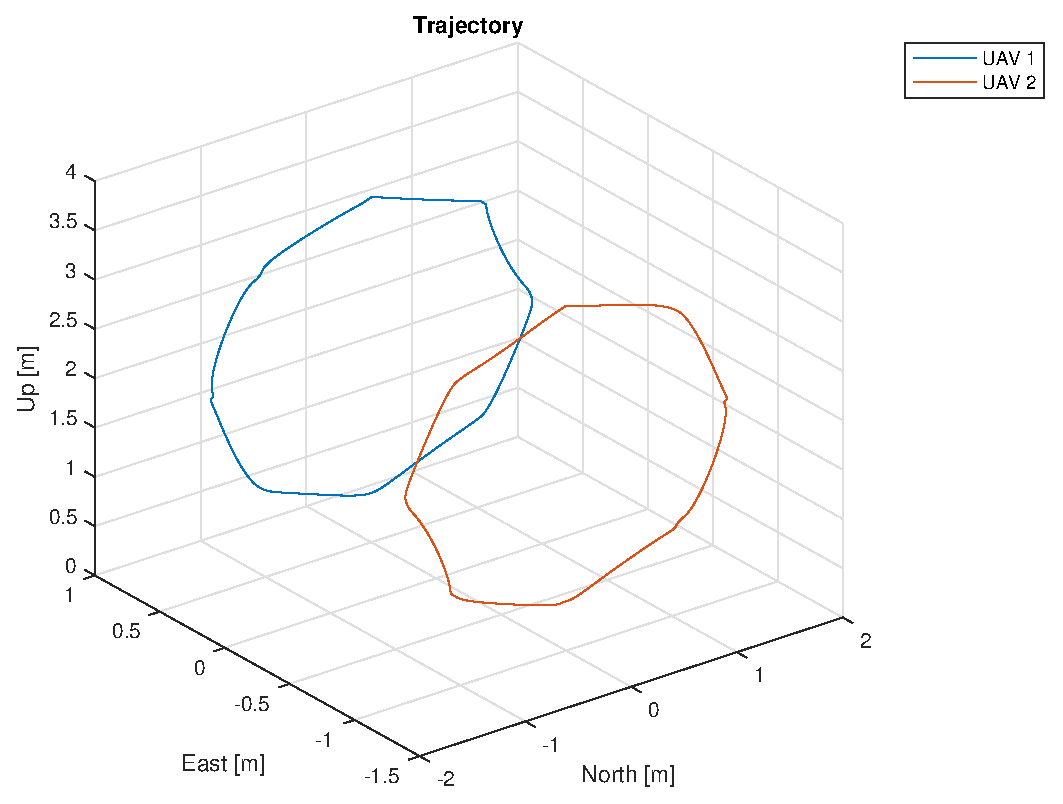
\includegraphics[width=0.7\textwidth]{chapters/chapter-04/figures/trajectory.eps}
\caption{Trajectory}
\label{fig:trajectory}
\end{figure}

Both drones start in the upper point of their circle and then they move along the
trajectory in opposite directions. The mission terminates when both drones reach
their starting point.
The evolution of the trajectory in time of the first drone can be seen in the Figure
\ref{fig:trajectory_during_time}.

\begin{figure}
\centering
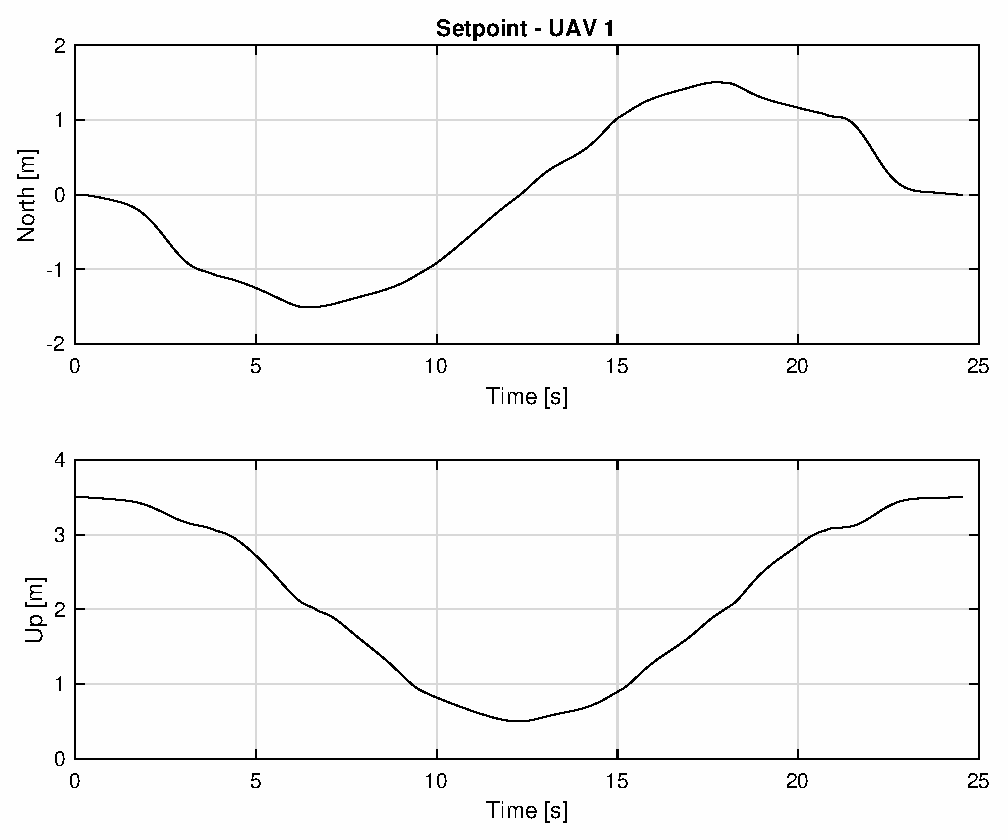
\includegraphics[width=0.7\textwidth]{chapters/chapter-04/figures/pos.eps}
\caption{Evolution of the trajectory in time of the first drone}
\label{fig:trajectory_during_time}
\end{figure}

How the two drones follow their trajectory is shown in the Figures
\ref{fig:following_1} and \ref{fig:following_2}.

\begin{figure}
\centering
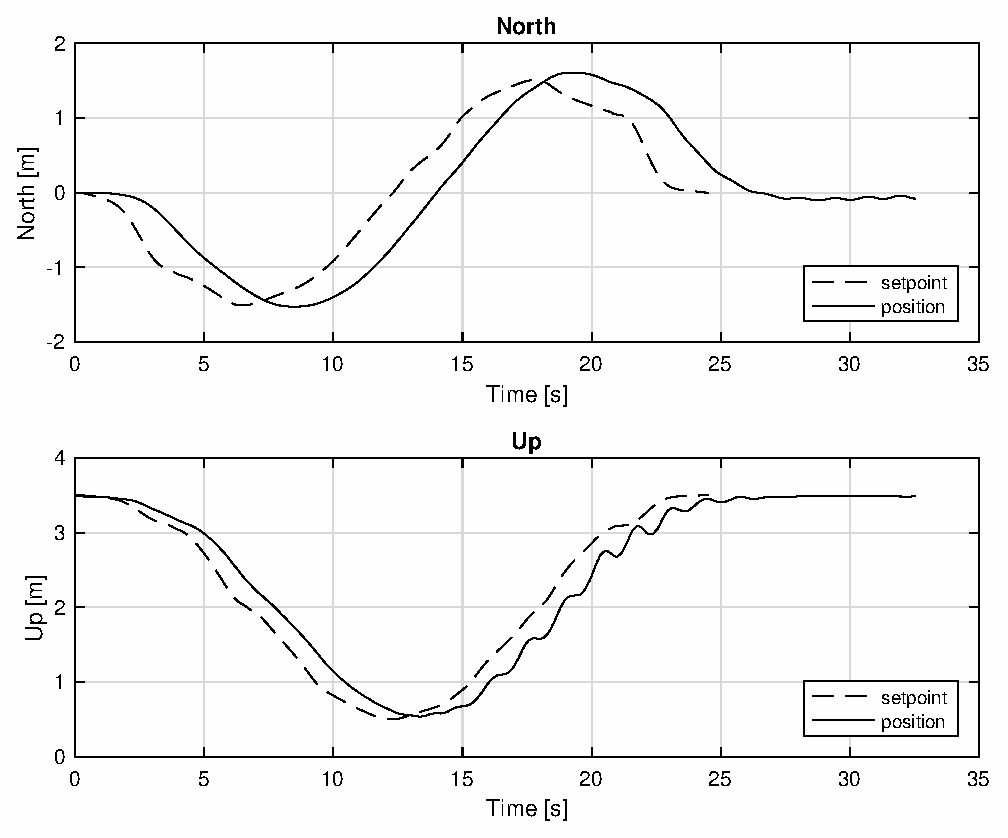
\includegraphics[width=0.7\linewidth]{chapters/chapter-04/figures/following_1.eps}
\caption{Target following drone 1}
\label{fig:following_1}
\end{figure}

\begin{figure}
\centering
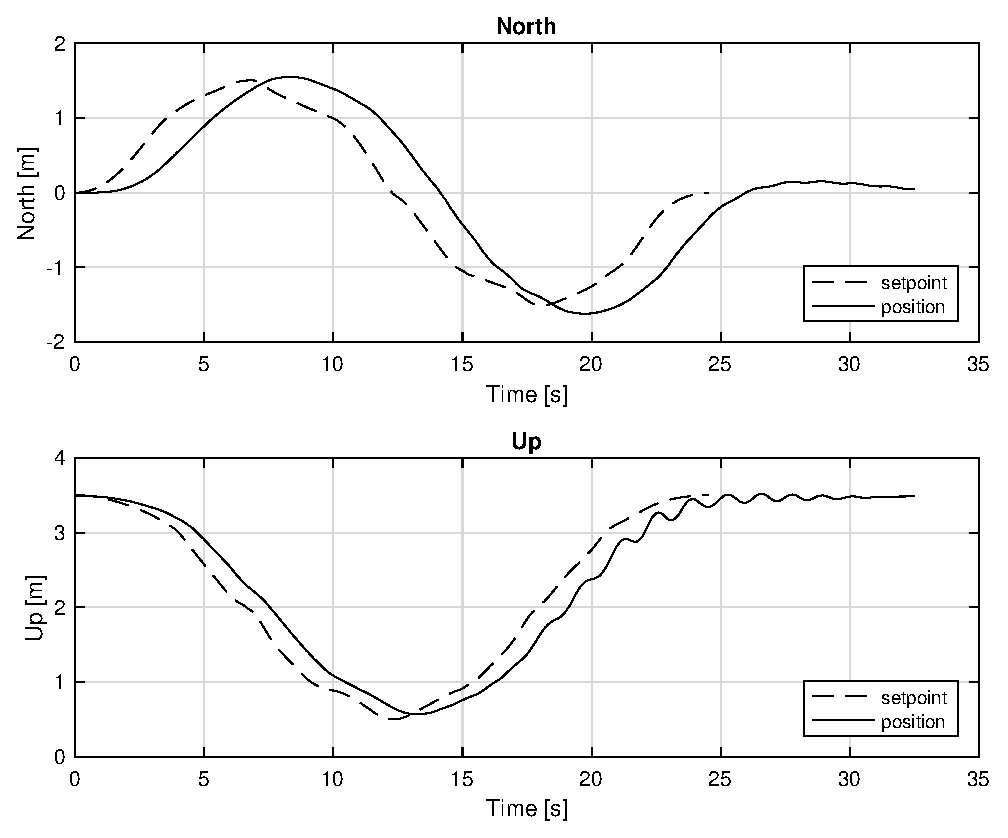
\includegraphics[width=0.7\linewidth]{chapters/chapter-04/figures/following_2.eps}
\caption{Target following drone 2}
\label{fig:following_2}
\end{figure}

There are some delays due to the fact that the autopilot needs time to follow the target,
but the drones can follow if successfully.
In fact, they arrive at their final position at the same time.

\begin{figure}
\centering
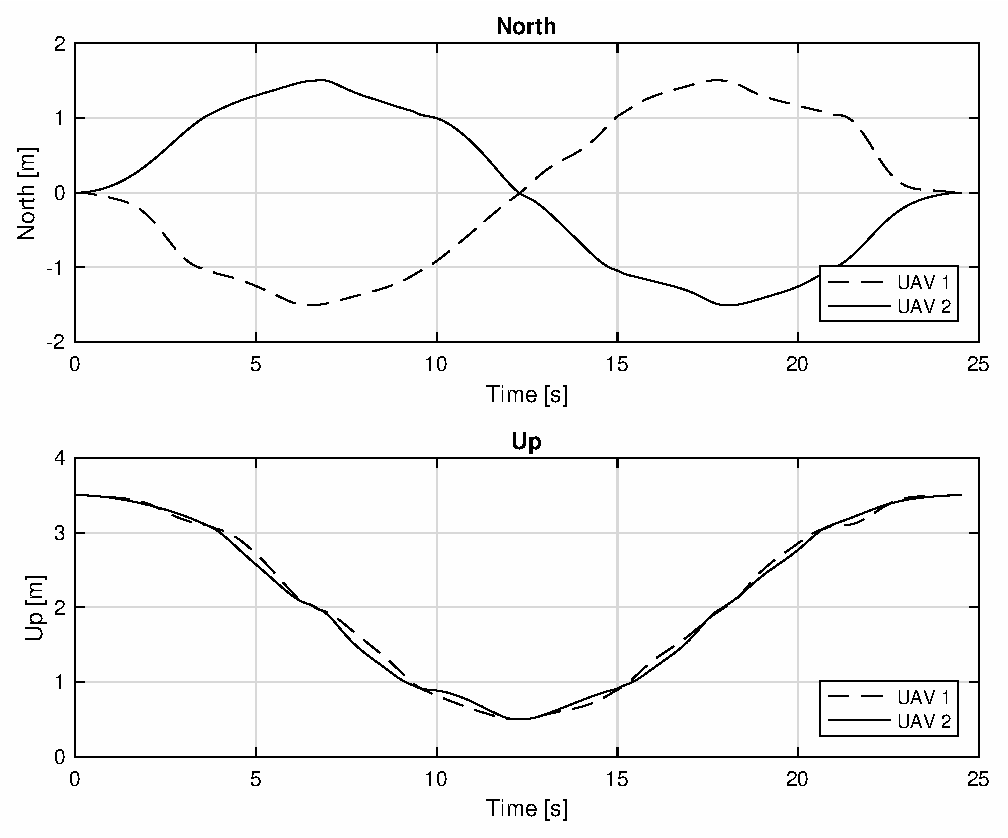
\includegraphics[width=0.7\textwidth]{chapters/chapter-04/figures/overlapped.eps}
\caption{Positions of the two drones in time}
\label{fig:overlapped}
\end{figure}

If we also consider the Figure \ref{fig:overlapped}, we can see that both drones
are synchronized during the execution of the mission. In the next cases, we will
add disturbances in order to make the effects of the algorithm more evident.


\section{First disturbance}
In this scenario, we use the same trajectory as before (Figure \ref{fig:trajectory}),
but in this case we stop one of the two drones and the other will follow it.
The Figure \ref{fig:disturbance} shows the disturbance applied to the first drone at time 11s.

\begin{figure}
\centering
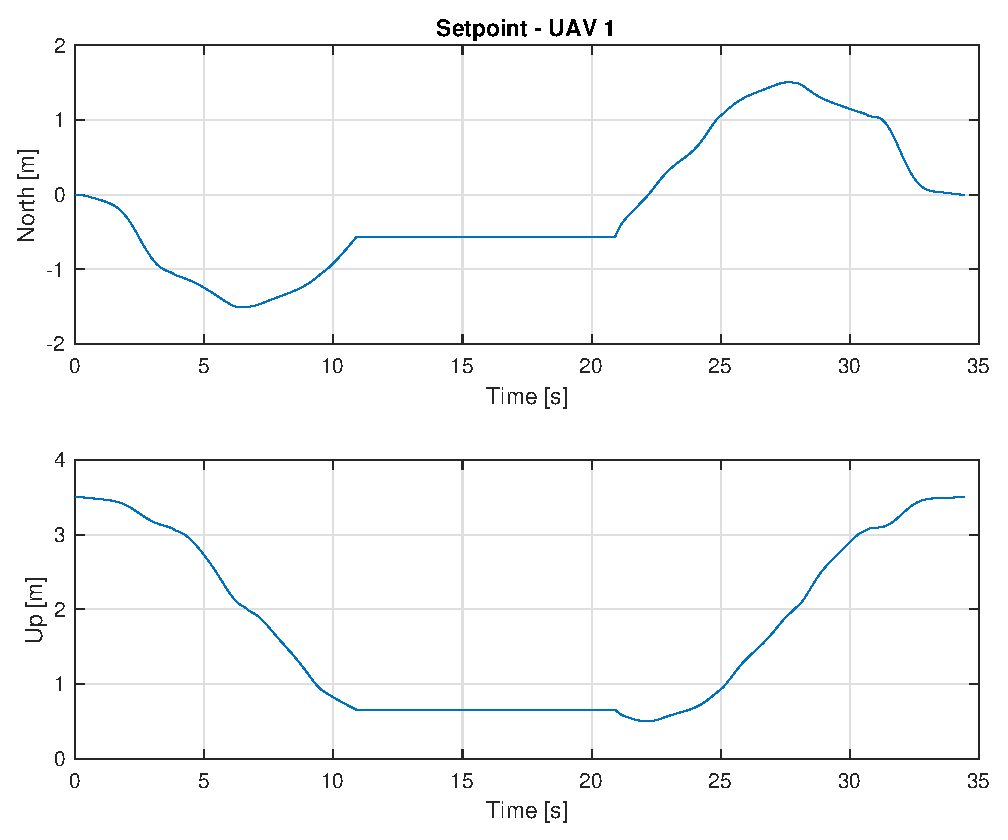
\includegraphics[width=0.7\textwidth]{chapters/chapter-04/figures/pos_1.eps}
\caption{Disturbance}
\label{fig:disturbance}
\end{figure}

We can now see how the two drones execute the mission. The second drone tries to
go on when the first is interrupted, but then the consensus stops it. The plots are
shown in the Figures \ref{fig:following_1_1} and \ref{fig:following_2_1}.

\begin{figure}
\centering
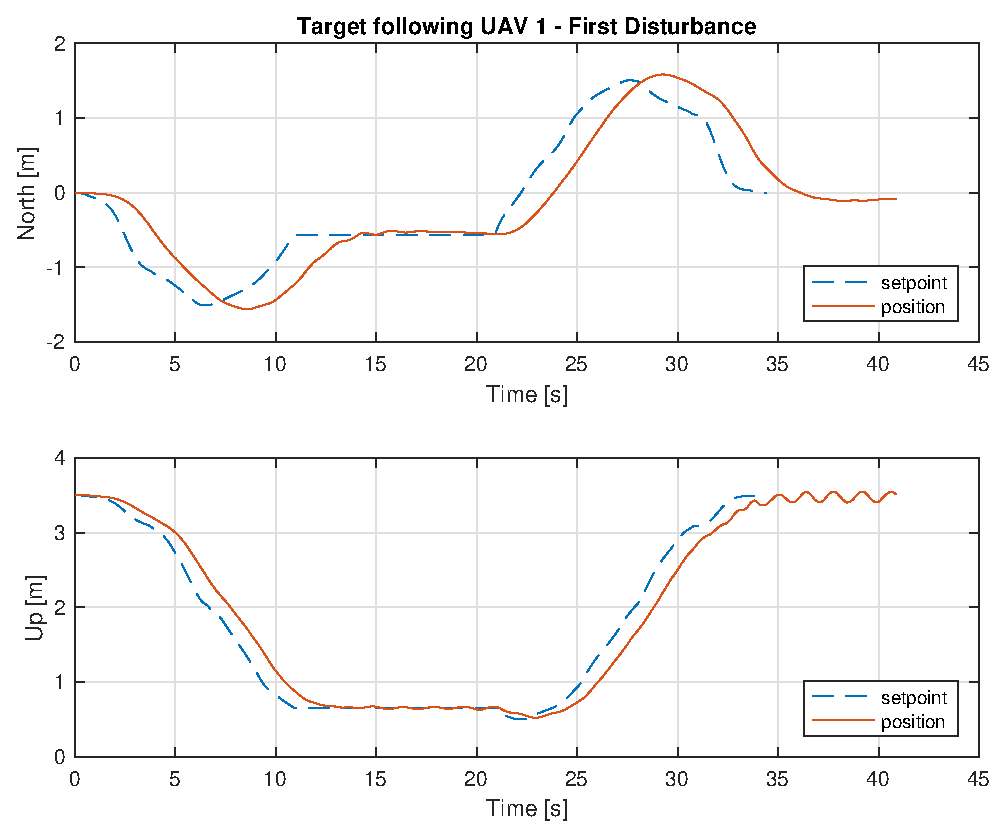
\includegraphics[width=0.7\linewidth]{chapters/chapter-04/figures/following_1_1.eps}
\caption{Target following drone 1}
\label{fig:following_1_1}
\end{figure}

\begin{figure}
\centering
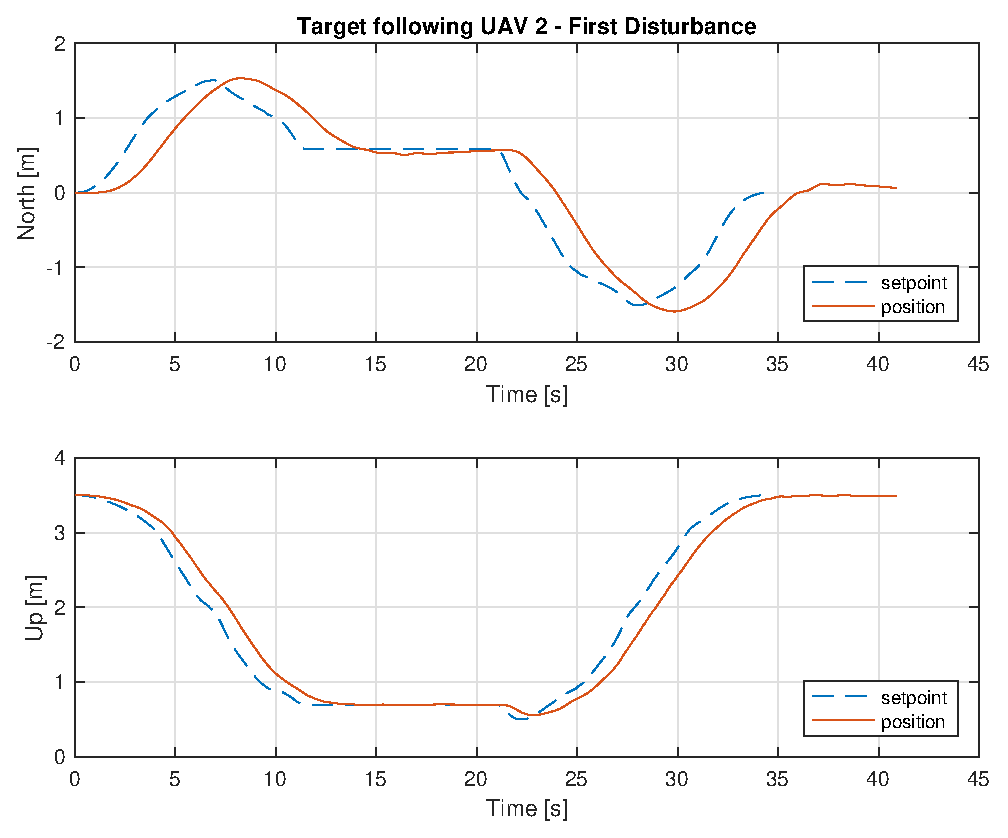
\includegraphics[width=0.7\linewidth]{chapters/chapter-04/figures/following_2_1.eps}
\caption{Target following drone 2}
\label{fig:following_2_1}
\end{figure}

Finally, the Figure \ref{fig:overlapped_1} is a graph representing the overlapped
positions of the two drones.


\begin{figure}
\centering
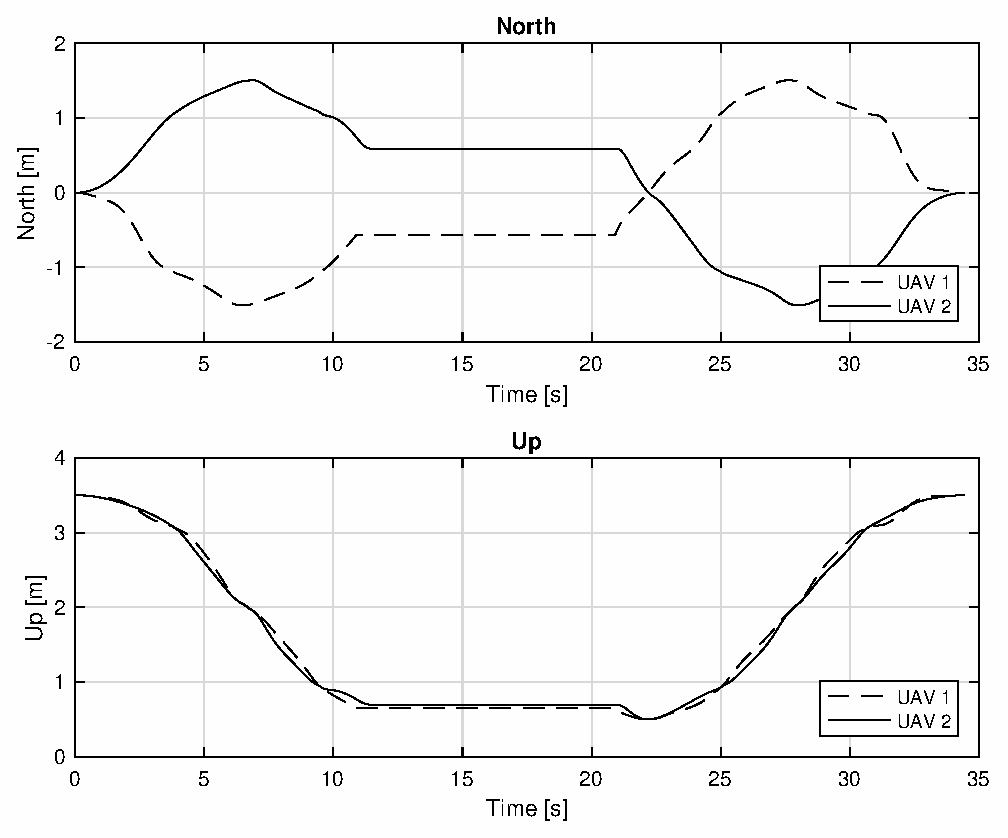
\includegraphics[width=0.7\textwidth]{chapters/chapter-04/figures/overlapped_1.eps}
\caption{Positions of the two drones in time}
\label{fig:overlapped_1}
\end{figure}


\section{Second disturbance}
The trajectory used is always the same (Figure \ref{fig:trajectory}), but this time
the disturbance is different. Now we force one drone to go back through the trajectory
which has travelled so far.
After the disturbance, the drone can resume the trajectory and complete the mission.
We can see the effect of the disturbance on the trajectory in the Figure \ref{fig:disturbance_2}.

\begin{figure}
\centering
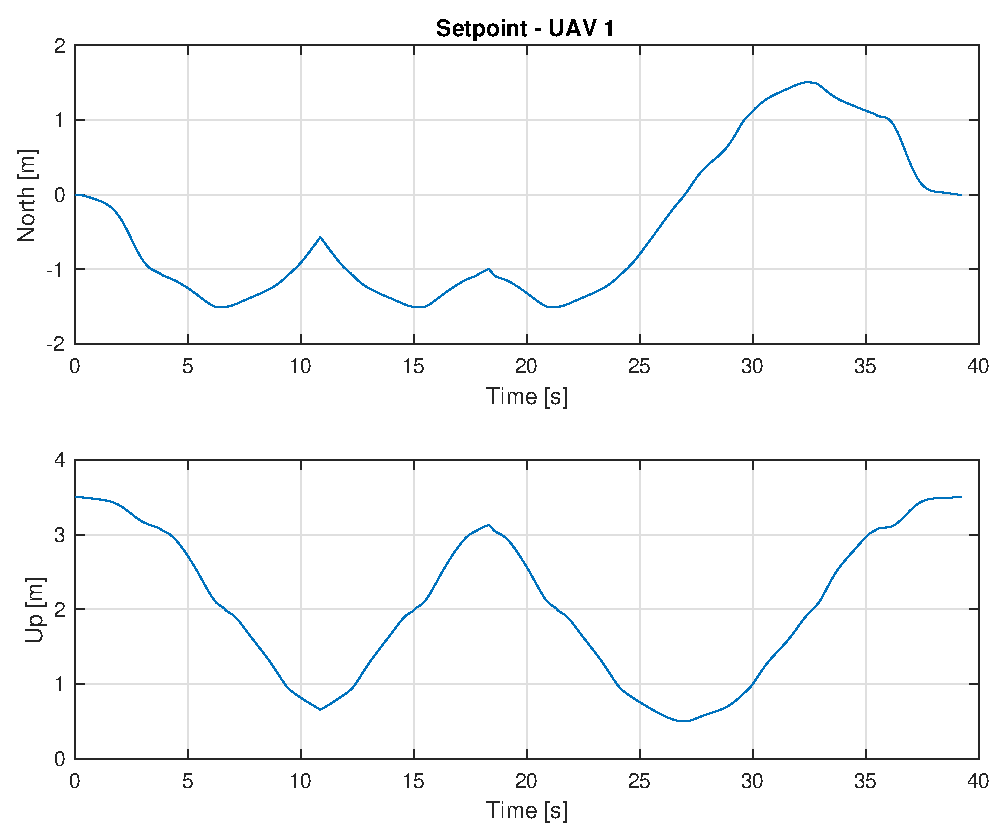
\includegraphics[width=0.7\textwidth]{chapters/chapter-04/figures/pos_2.eps}
\caption{Disturbance}
\label{fig:disturbance_2}
\end{figure}

At time 11s the disturbance starts and the drone begins to go back. At time 26s,
the drone has returned to the position where the disturbance is started.

In this situation, the other drone recognizes that the other machine is going backward
for an unknown reason and starts to follow it. We can see how the mission is done
by the two drones in the Figures \ref{fig:following_1_2} and \ref{fig:following_2_2}.

\begin{figure}
\centering
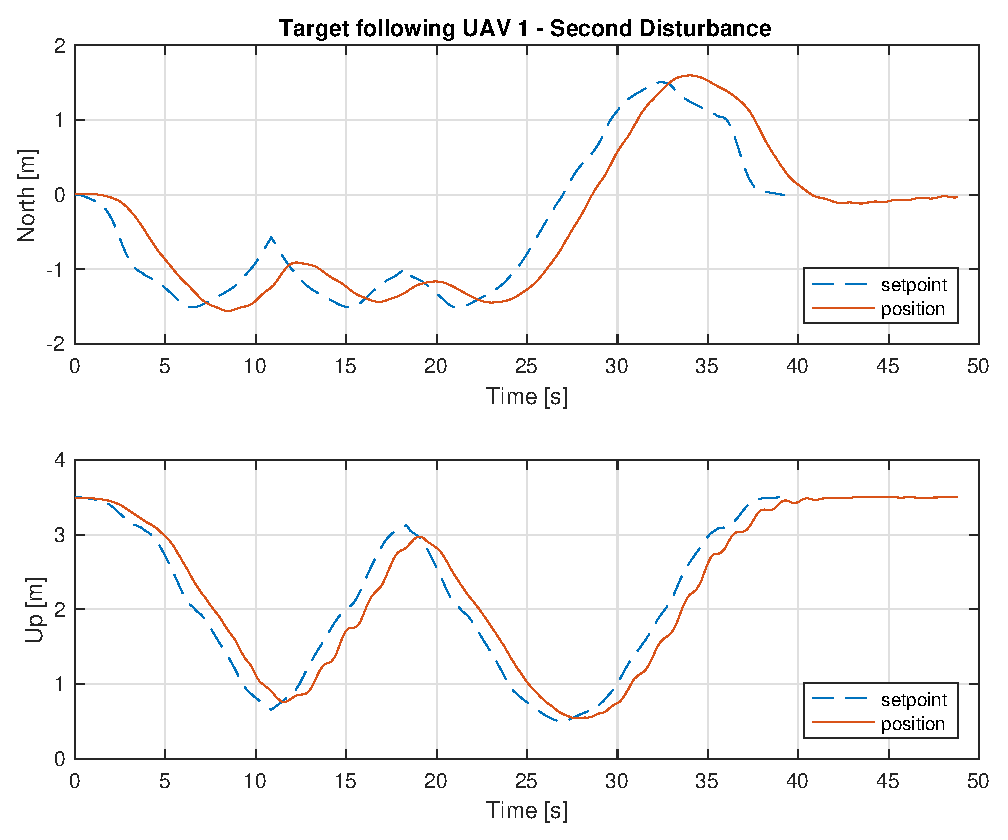
\includegraphics[width=0.7\linewidth]{chapters/chapter-04/figures/following_1_2.eps}
\caption{Target following drone 1}
\label{fig:following_1_2}
\end{figure}

\begin{figure}
\centering
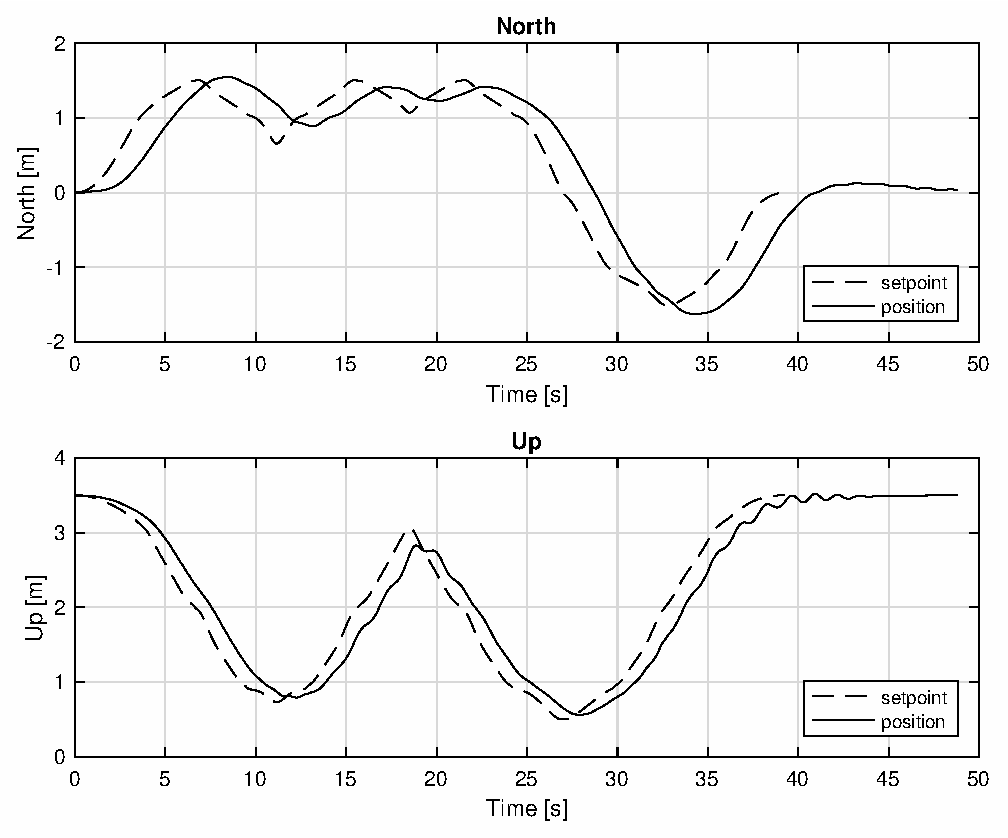
\includegraphics[width=0.7\linewidth]{chapters/chapter-04/figures/following_2_2.eps}
\caption{Target following drone 2}
\label{fig:following_2_2}
\end{figure}

\begin{figure}
\centering
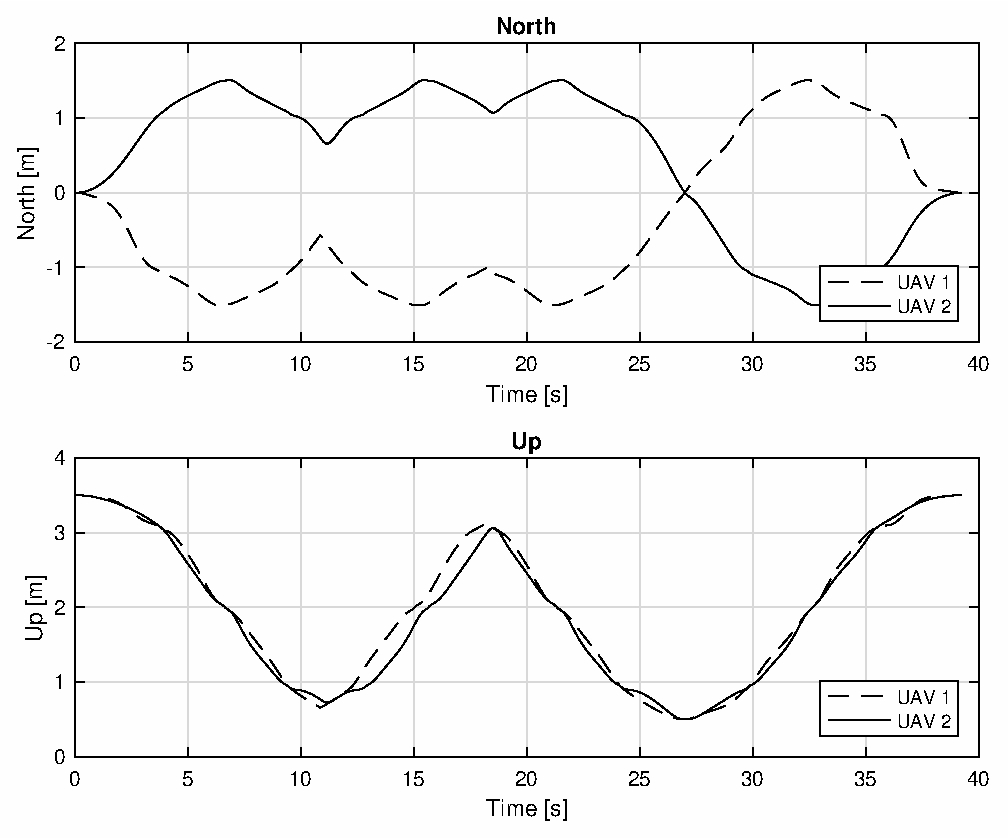
\includegraphics[width=0.7\textwidth]{chapters/chapter-04/figures/overlapped_2.eps}
\caption{Positions of the two drones in time}
\label{fig:overlapped_2}
\end{figure}


Finally, the Figure \ref{fig:overlapped_2}, is a graph representing the overlapped
positions of the two drones.


%%%%%%%%%%%%%%%%%%%%%%%%%%%%%% Chapter 5
\chapter{Experimental results\label{chap:experimental_results}}
In this chapter we present the results obtained applying the simulations done in the
previous chapter to a real system.

We want to highlight that the algorithm works even in the real system
and the results obtained are compatible with the simulated ones.
In this scenario, we need to take into account that the network is not ideal and
the data may suffer delays and inaccuracy due to the complex clock synchronization
of the machines involved in the experiment.

As in chapter \ref{chap:simulation_results}, we will run the experiment three times.
First, the formation has to follow the trajectory without disturbances.
The second time, we run the algorithm and then we stop one of the drones, while the other one
will try to go on, but then it stops.
Third, we apply a disturbance which forces one of the drones to go back following
in the reverse order its trajectory. The other drone just follows it, because it is
forced to preserve the formation.

The trajectory used is the same as the simulated one (\ref{fig:trajectory}), and
the drones start on the top points of their trajectory, following the circle in opposite
directions.
They must be symmetric and finish the mission at the same time.

We now present the three cases in detail.

\section{Trajectory following}
The two drones will follow the trajectory, as shown in the Figures \ref{fig:exp_following_1}
and \ref{fig:exp_following_2}.

\begin{figure}
\centering
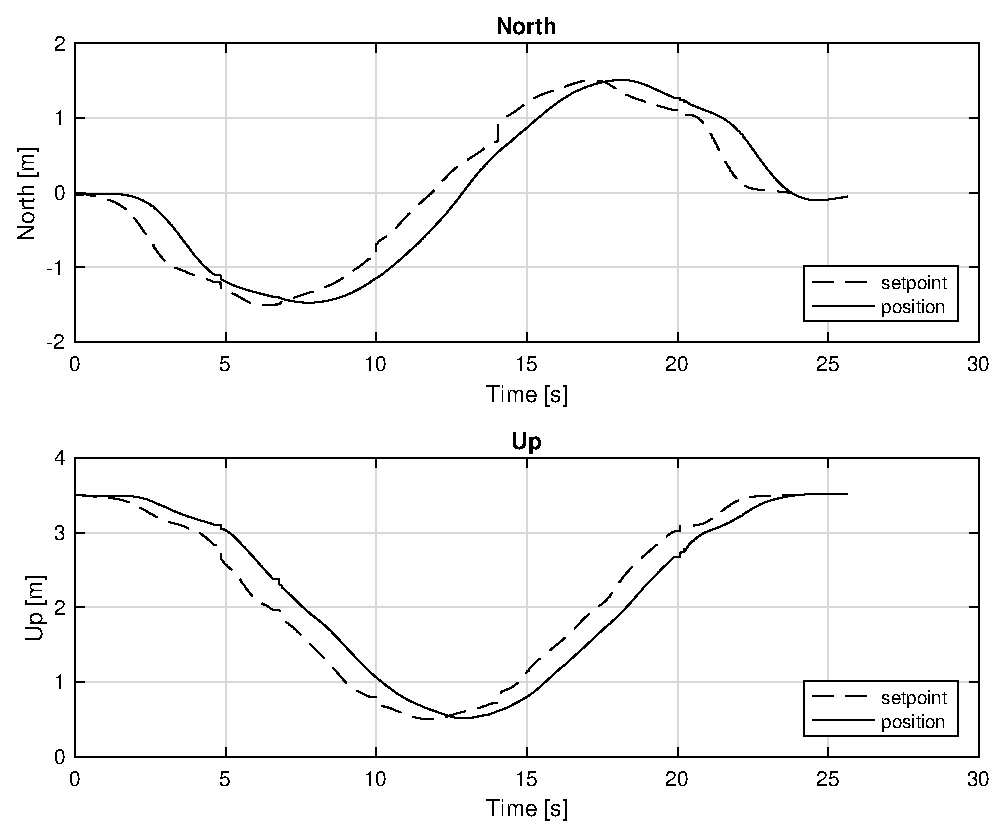
\includegraphics[width=0.7\linewidth]{chapters/chapter-05/figures/following_1.eps}
\caption{Target following drone 1}
\label{fig:exp_following_1}
\end{figure}

\begin{figure}
\centering
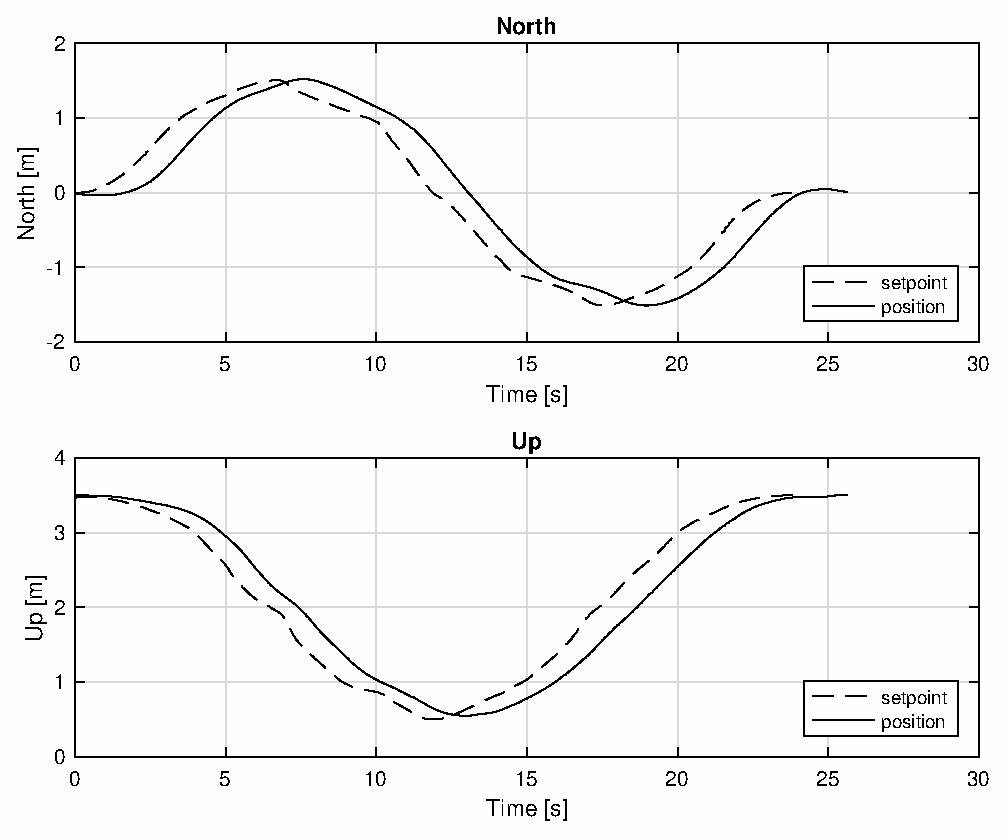
\includegraphics[width=0.7\linewidth]{chapters/chapter-05/figures/following_2.eps}
\caption{Target following drone 2}
\label{fig:exp_following_2}
\end{figure}

Even in this case, there are some delays due to the time needed to the autopilot to follow
the target, but the drones are capable of doing that.
The two drones stay synchronized during all the mission as we can see in the Figure
\ref{fig:exp_overlapped}.

\begin{figure}
\centering
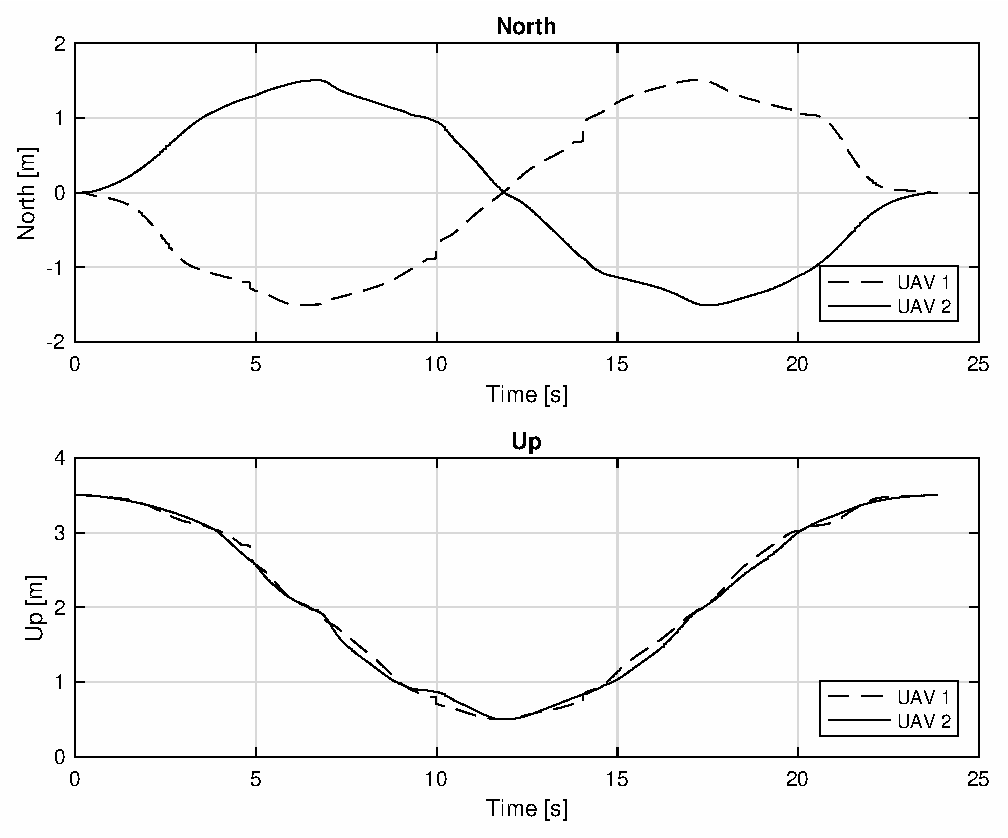
\includegraphics[width=0.7\textwidth]{chapters/chapter-05/figures/overlapped.eps}
\caption{Two drones positions over time}
\label{fig:exp_overlapped}
\end{figure}


\section{First disturbance}

When we add a disturbance to one of the drones, the algorithm rejects it and preserves
the formation. In this experiment we introduce the disturbance a time 6s and it
terminates after 10s. We see the mission in the Figures \ref{fig:exp_following_1_1}
and \ref{fig:exp_following_2_1}.

\begin{figure}
\centering
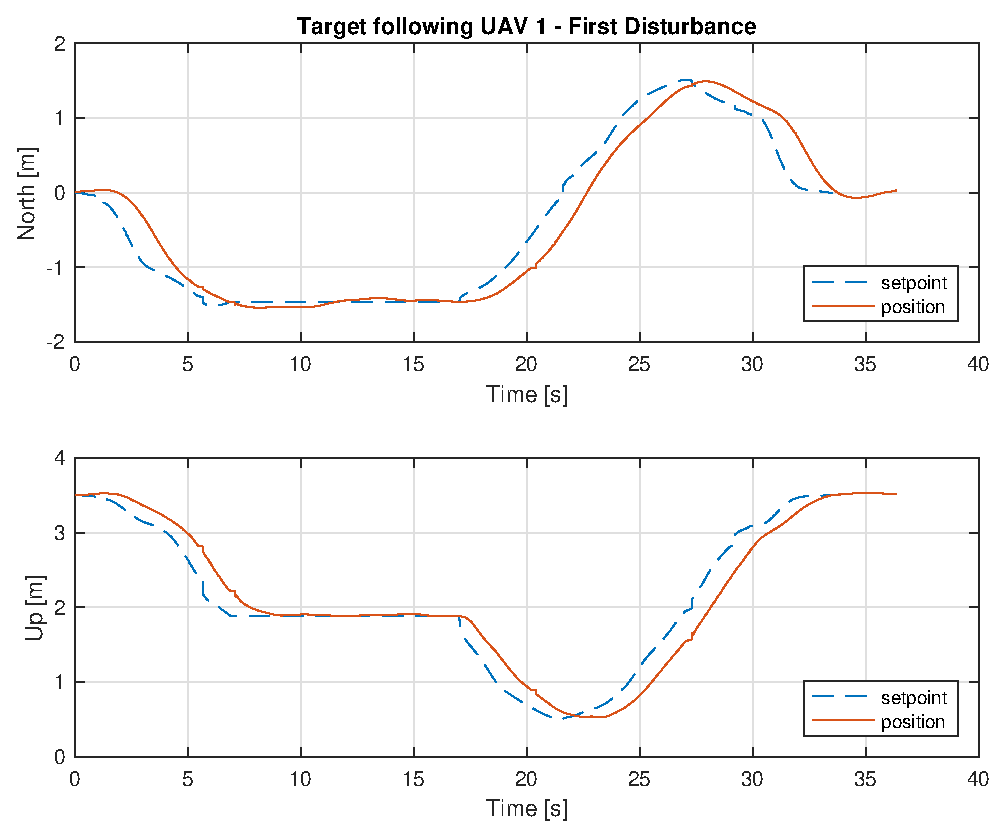
\includegraphics[width=0.7\linewidth]{chapters/chapter-05/figures/following_1_1.eps}
\caption{Target following drone 1}
\label{fig:exp_following_1_1}
\end{figure}

\begin{figure}
\centering
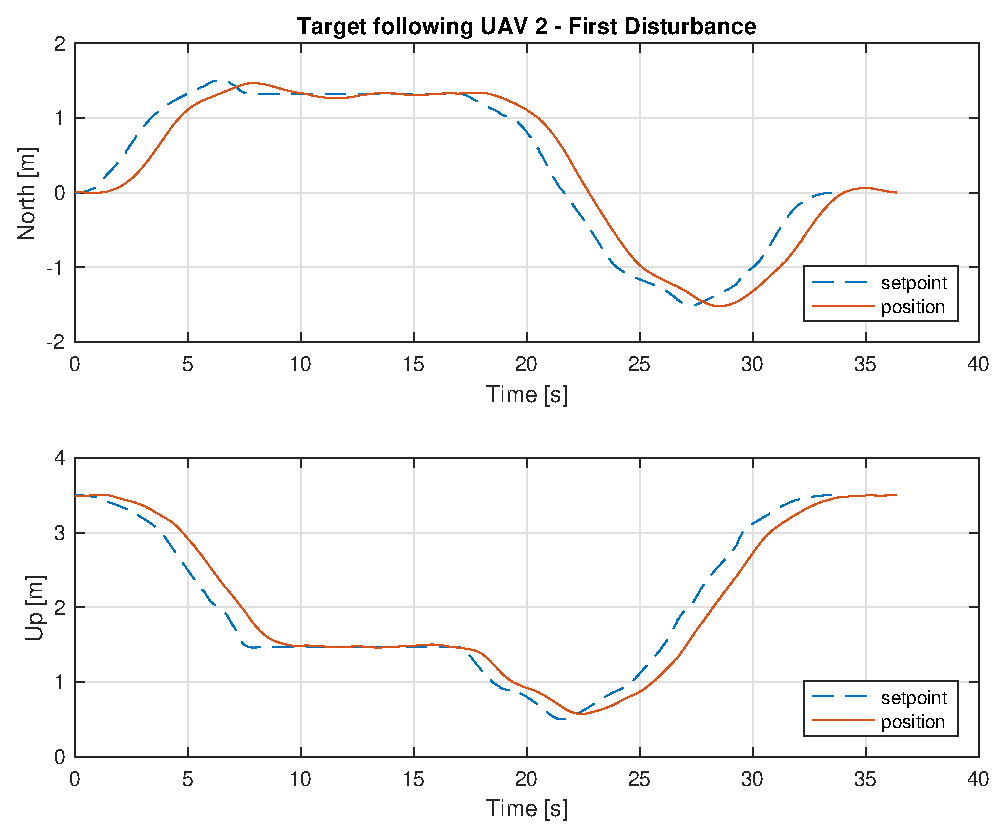
\includegraphics[width=0.7\linewidth]{chapters/chapter-05/figures/following_2_1.eps}
\caption{Target following drone 2}
\label{fig:exp_following_2_1}
\end{figure}

The disturbance causes the other drone to stop and wait until the disturbance
is finished. We can see the synchronization in the Figure \ref{fig:exp_overlapped_1}.

\begin{figure}
\centering
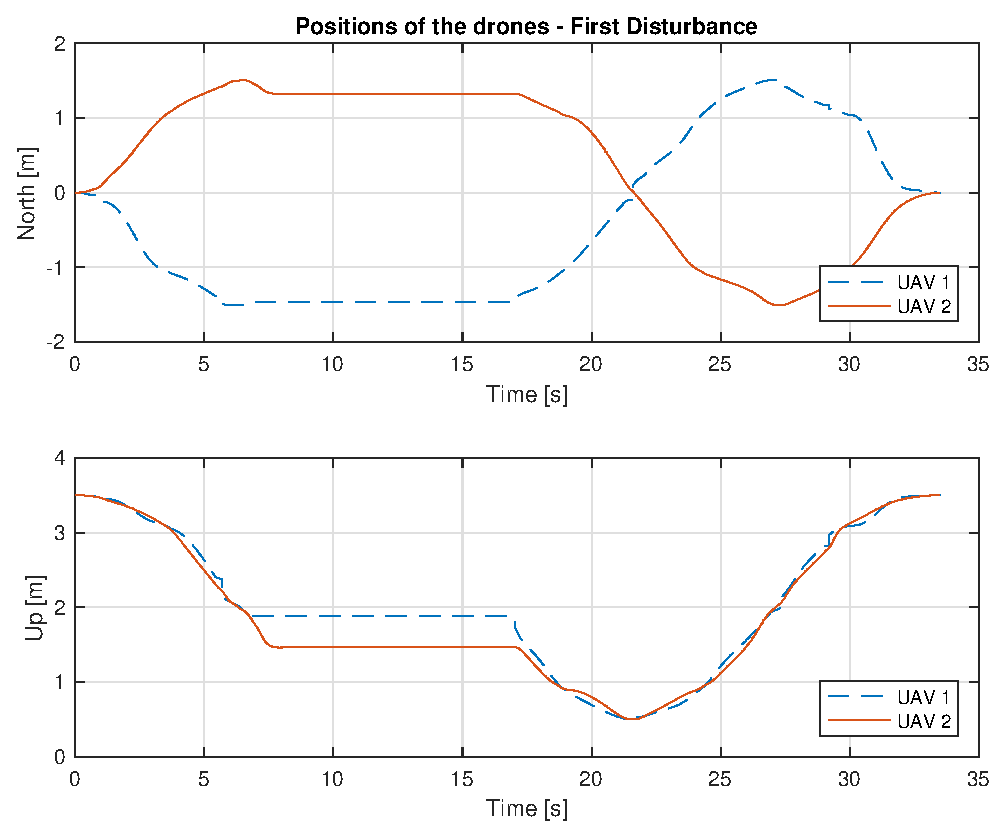
\includegraphics[width=0.7\textwidth]{chapters/chapter-05/figures/overlapped_1.eps}
\caption{Two drones positions over time}
\label{fig:exp_overlapped_1}
\end{figure}

\section{Second disturbance}
The last disturbance we show is the one which forces a drone to go back through the
trajectory. We can see how the setpoints are changed when the disturbance is active
and how the drones follow them. The Figures \ref{fig:exp_following_1_2}
and \ref{fig:exp_following_2_2} present the results.

\begin{figure}
\centering
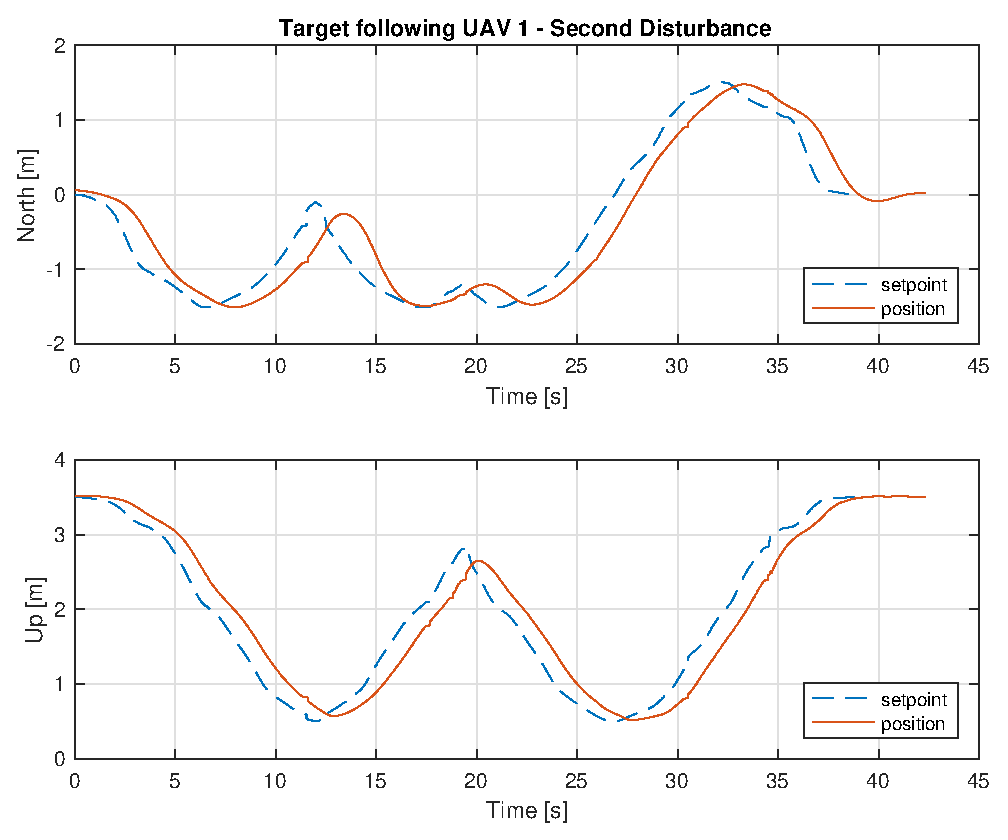
\includegraphics[width=0.7\linewidth]{chapters/chapter-05/figures/following_1_2.eps}
\caption{Target following drone 1}
\label{fig:exp_following_1_2}
\end{figure}

\begin{figure}
\centering
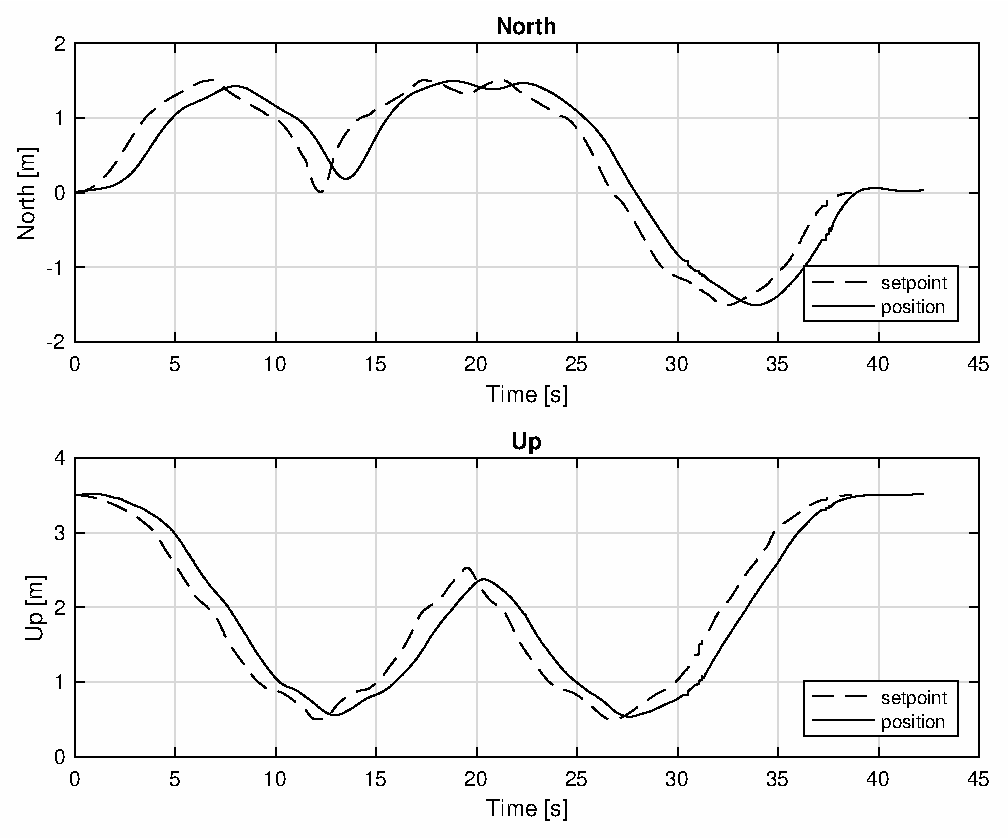
\includegraphics[width=0.7\linewidth]{chapters/chapter-05/figures/following_2_2.eps}
\caption{Target following drone 2}
\label{fig:exp_following_2_2}
\end{figure}

The disturbance causes the other drone to stop and go back, following the other,
until the disturbance is finished.
We can see the synchronization in the Figure \ref{fig:exp_overlapped_2}.

\begin{figure}
\centering
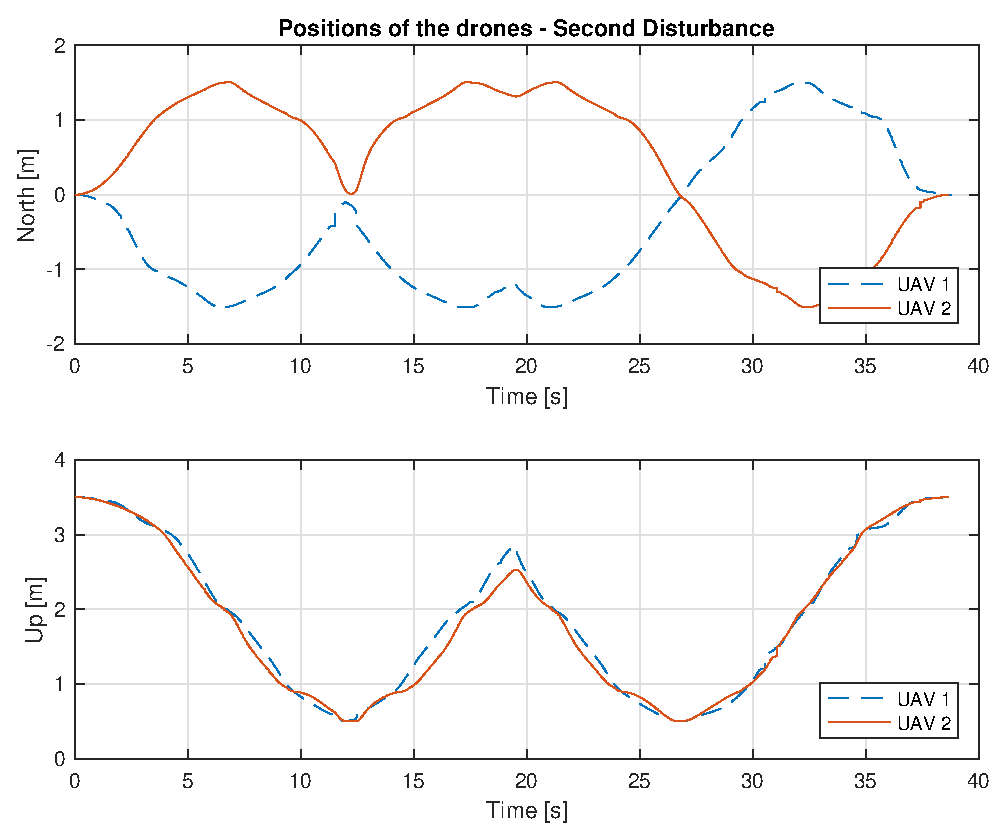
\includegraphics[width=0.7\textwidth]{chapters/chapter-05/figures/overlapped_2.eps}
\caption{Two drones positions over time}
\label{fig:exp_overlapped_2}
\end{figure}

The experimental results are less accurate than the simulated ones,
but the overall behaviour is preserved. Indeed, if we compare the results, we
can see that the formation is maintained in both cases. The plots are very similar
even if the simulated model of the drones does not reflect the real drones and even if
the drones used are heterogeneous.


%%%%%%%%%%%%%%%%%%%%%%%%%%%%%% Conclusion
\chapter*{Conclusions}
\addcontentsline{toc}{chapter}{Conclusions}
\markboth{Conclusions}{Conclusions}
%The conclusions must recall the field of work, the purpose of the thesis, what has been done and an evaluation of the obtained results.
%Furthermore, the conclusion must also emphasize the future prospects and must show how to move forward in the study area.

The results obtained in our experiments can be applied in many fields in which
a formation of UAVs has to operate.
In this thesis, we have shown how the consensus algorithm is deployed on a real
system and which performances can be achieved.

The implementation allows us to plan and fulfill a cooperative
mission in which the synchronization is one of the most important aspects.
The system is robust to network delays and loss of packets and to unexpected failures
of the vehicles involved.
Moreover, the formation, if equipped with an obstacle avoidance algorithm,
overcomes the presence of unexpected obstacles during the execution of the mission.

Further studies can be carried on in order to integrate recovery procedures in case
of network failures or the loss of a machine.
It is possible to develop obstacle avoidance algorithms or any kind of online procedures
acting directly on the free parameters of the algorithm presented.
In particular, it is possible to change the values of $\ddot{\gamma_d}$ and $\dot{\gamma_d}$,
in order to modify the velocity of the execution of the mission. These two values
can be also used to build more complex functionalities on top of the consensus algorithm.


%%%%%%%%%%%%%%%%%%%%%%%%%%%%%% Bibliography
\bibliographystyle{plain}
\bibliography{bibliography}

%%%%%%%%%%%%%%%%%%%%%%%%%%%%%% END OF THE DOCUMENT
\end{document}
